\part{Data Mining}


    \section{Justification of the Test Design}

        In the context of data mining with the specific goal of building predictive models to maintain obesity rates below 20\%, we have chosen to allocate 20\% of the data for testing and 80\% for training. This strategic distribution balances the need for thorough model evaluation with effective pattern recognition.

        \subsection{Equilibrium Between Evaluation and Learning}
            The 80-20 data split is intentional, aiming to create a balance between assessing the models and training them with comprehensive data. This helps prevent the models from becoming too specialized to the training data, thus enabling good generalization to unseen data.

        \subsection{Linear Model Rationalization}
            In the linear model context, having 80\% of the data for training enables the model to establish intricate relationships between the predictors and obesity rates. The remaining 20\% serves as an independent test set, ensuring that the model avoids overfitting and effectively predicts obesity rates below 20\%.

        \subsection{Logistic Model Justification}
            For logistic models, which are good for binary classification, the 80-20 split is also justified. The model learns from the training set while the testing set scrutinizes its ability to classify instances it hasn't seen, particularly those exceeding the 20\% obesity threshold.

        \subsection{Ensuring Uniformity and Integrity}
            Using a consistent data split ratio for both models introduces uniformity to the evaluation process. This ensures parallel conditions for assessing both models and avoids unintended disparities in performance evaluation.

        \subsection{Validating Generalization and Reliability}
            Reserving 30\% of the data for testing allows us to rigorously evaluate the models' ability to generalize to new, unseen data, thereby confirming their reliability in real-world scenarios.

        \subsection{Summary}
            In summary, the 80-20 data split is a strategic choice that aligns with industry best practices. It provides a balanced approach for robust training and effective evaluation, aiming to produce models that can maintain obesity rates below the targeted 20\%.


    \section{Conduct data mining}

        \subsection{Model Tuning for Improved Precision}

            All subsequent models discussed have been rigorously tuned to enhance their precision score. The metric of precision has been deliberately selected for its pivotal role in emphasizing the accurate prediction of true positives. In the context of our study, where the goal is to identify genuine cases that align with our target, precision stands out as a quintessential metric. Misclassifying a negative instance as a positive one could lead to resource misallocation or misinformed decisions. Therefore, achieving a higher precision score ensures that our model's positive predictions are both reliable and trustworthy.

        \subsection{Models}

            \paragraph{Decision Tree}
                \begin{figure}[H]
                        \centering
                        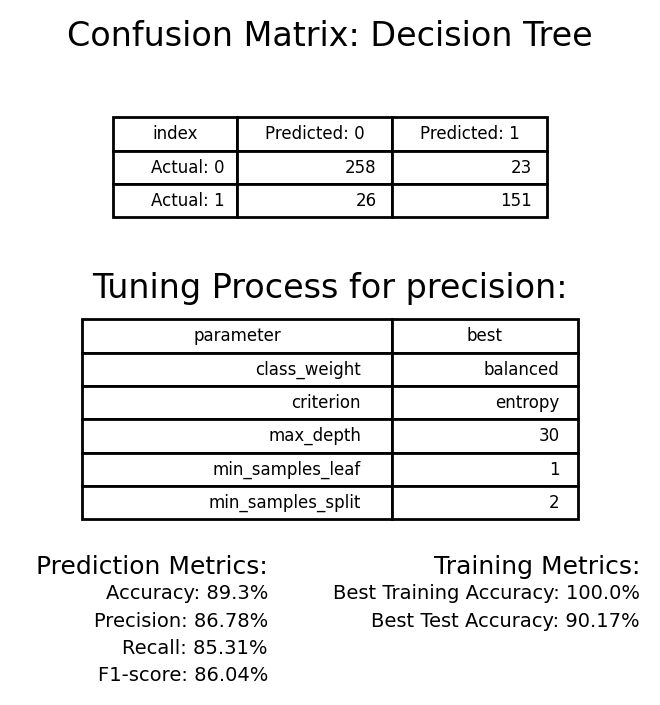
\includegraphics[scale=1]{images/dm_confu_mat_deci_tree}
                        \caption{Confusion Matrix and best parameters.}
                        \label{fig:dm-decision-tree}
                \end{figure}
                \begin{figure}[H]
                        \centering
                        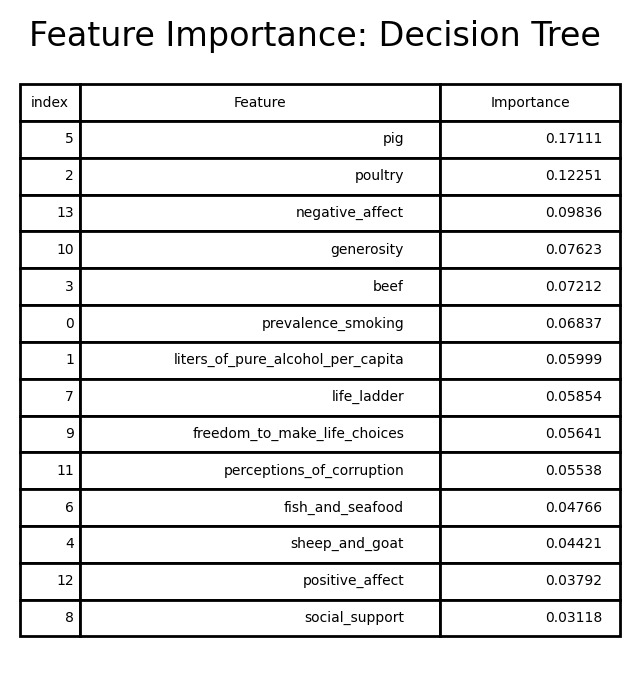
\includegraphics[scale=1]{images/dm_featu_imp_deci_tree}
                        \caption{Confusion Matrix and best parameters.}
                        \label{fig:dm-decision-tree-bp}
                \end{figure}

            \paragraph{Random Forest}
                \begin{figure}[H]
                        \centering
                        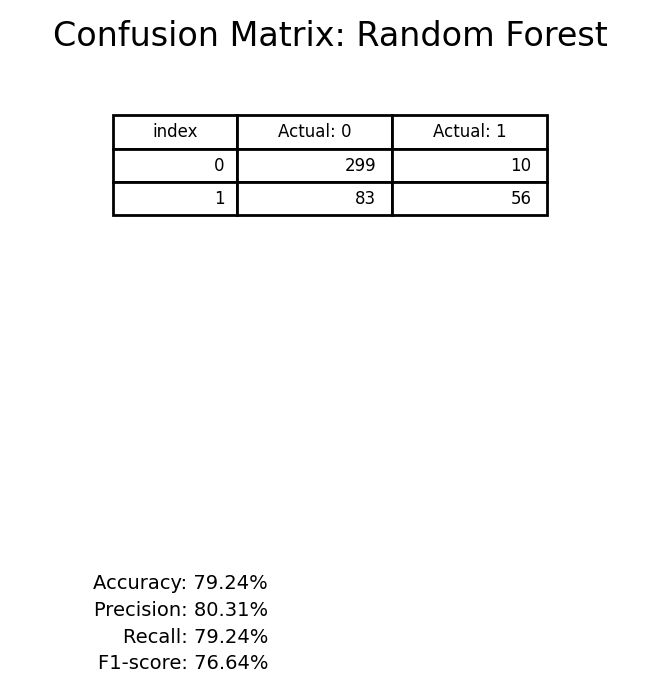
\includegraphics[scale=1]{images/dm_confu_mat_rand_fore}
                        \caption{Confusion Matrix and best parameters.}
                        \label{fig:dm-random-forest}
                \end{figure}
                \begin{figure}[H]
                        \centering
                        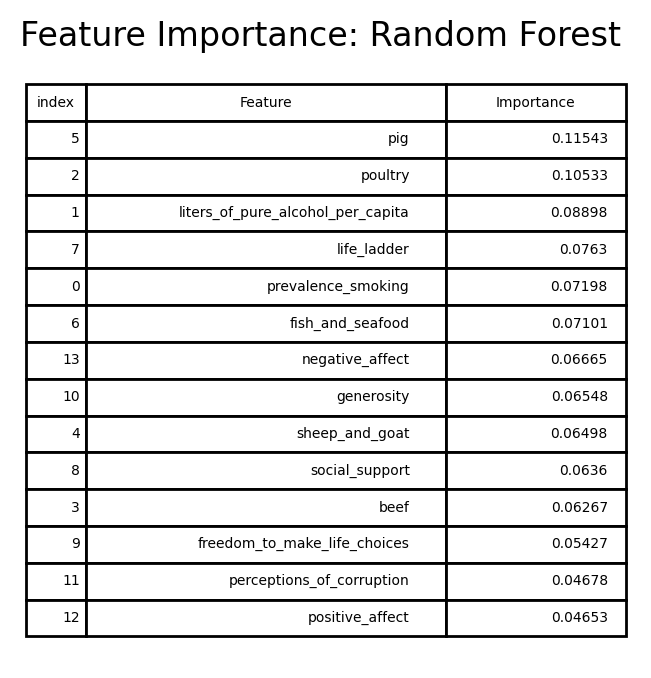
\includegraphics[scale=1]{images/dm_featu_imp_random_forest}
                        \caption{Confusion Matrix and best parameters.}
                        \label{fig:dm-random-forest-bp}
                \end{figure}

            \paragraph{Bernoulli Naive Bayes}
                \begin{figure}[H]
                        \centering
                        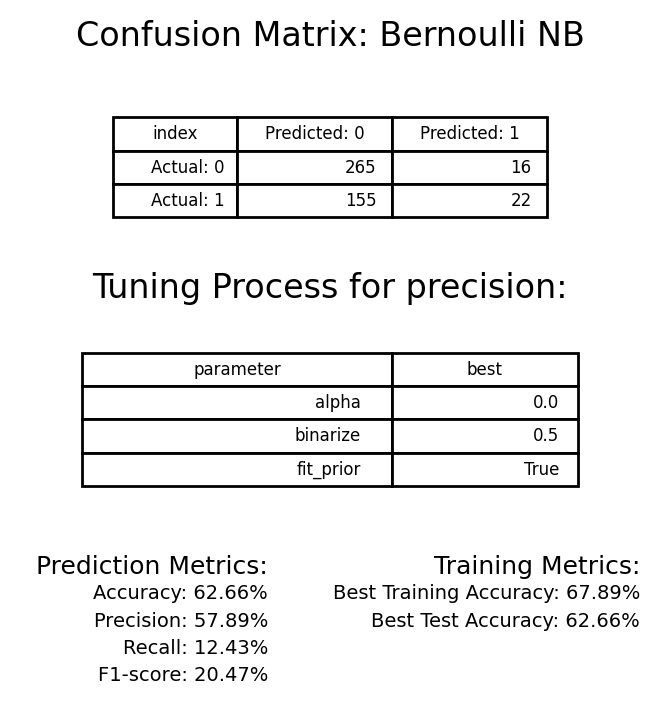
\includegraphics[scale=1]{images/dm_confu_mat_bern_nb}
                        \caption{Confusion Matrix and best parameters.}
                        \label{fig:dm-bernoulli-nb}
                \end{figure}
                \begin{figure}[H]
                        \centering
                        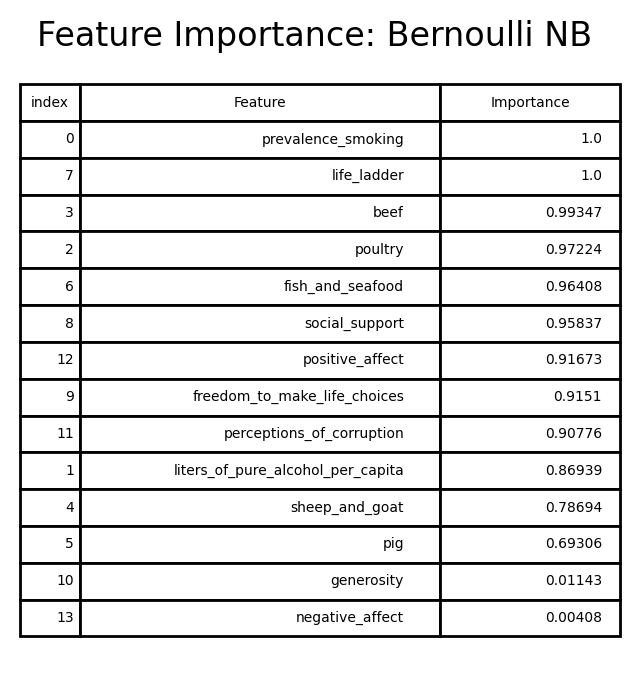
\includegraphics[scale=1]{images/dm_featu_imp_bern_nb}
                        \caption{Confusion Matrix and best parameters.}
                        \label{fig:dm-bernoulli-nb-bp}
                \end{figure}

            \paragraph{Gradient Boosting}
                \begin{figure}[H]
                        \centering
                        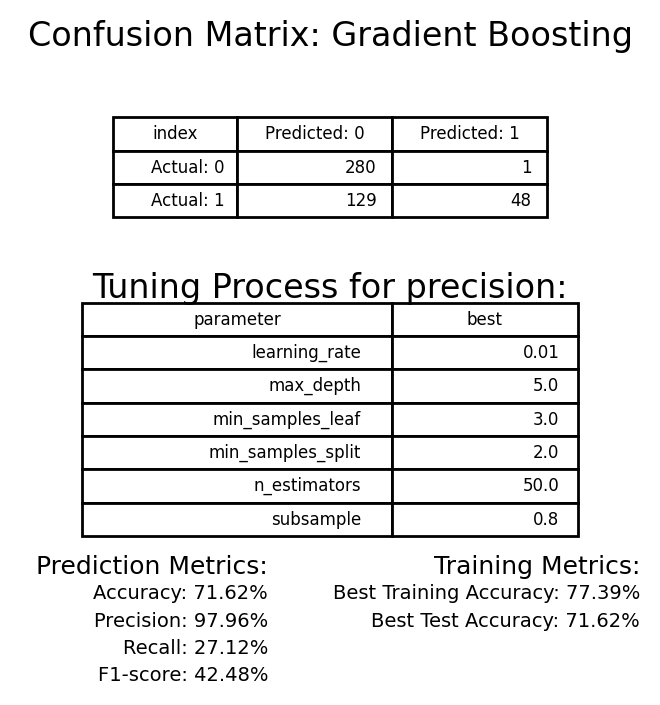
\includegraphics[scale=1]{images/dm_confu_mat_grad_boos}
                        \caption{Confusion Matrix and best parameters.}
                        \label{fig:dm-gradient-booting}
                \end{figure}
                \begin{figure}[H]
                        \centering
                        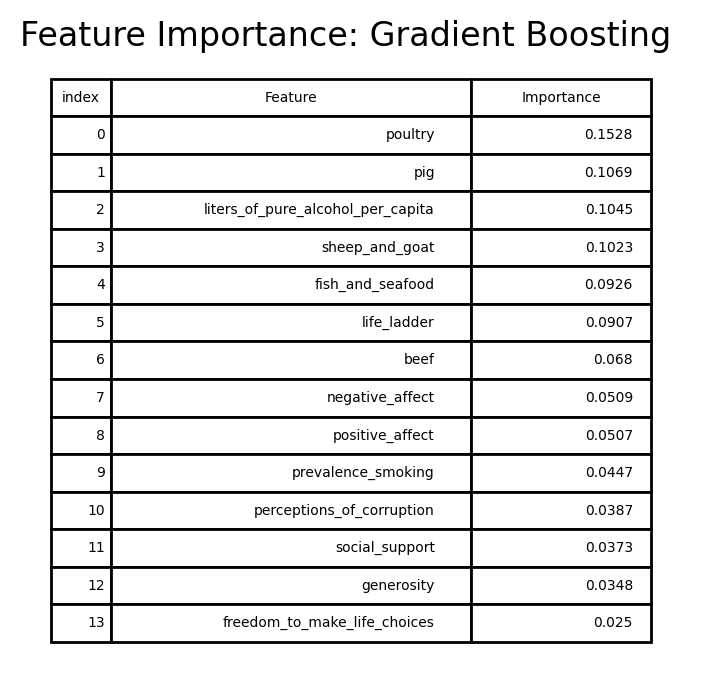
\includegraphics[scale=1]{images/dm_featu_imp_grad_boost}
                        \caption{Confusion Matrix and best parameters.}
                        \label{fig:dm-gradient-boosting-bp}
                \end{figure}

            \paragraph{Logistic Regression}
                \begin{figure}[H]
                        \centering
                        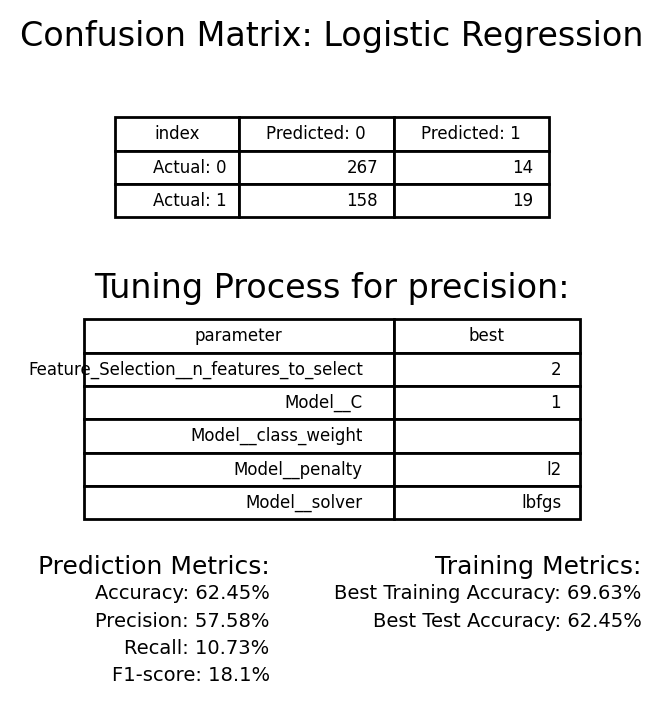
\includegraphics[scale=1]{images/dm_confu_mat_logi_regr}
                        \caption{Confusion Matrix and best parameters.}
                        \label{fig:dm-logistic-regression}
                \end{figure}
                \begin{figure}[H]
                        \centering
                        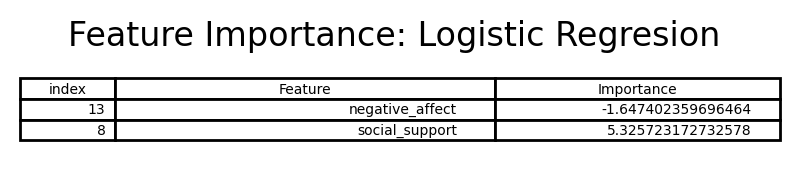
\includegraphics[scale=1]{images/dm_featu_imp_logi_regr}
                        \caption{Confusion Matrix and best parameters.}
                        \label{fig:dm-logistic-regression-bp}
                \end{figure}
                \begin{figure}[H]
                        \centering
                        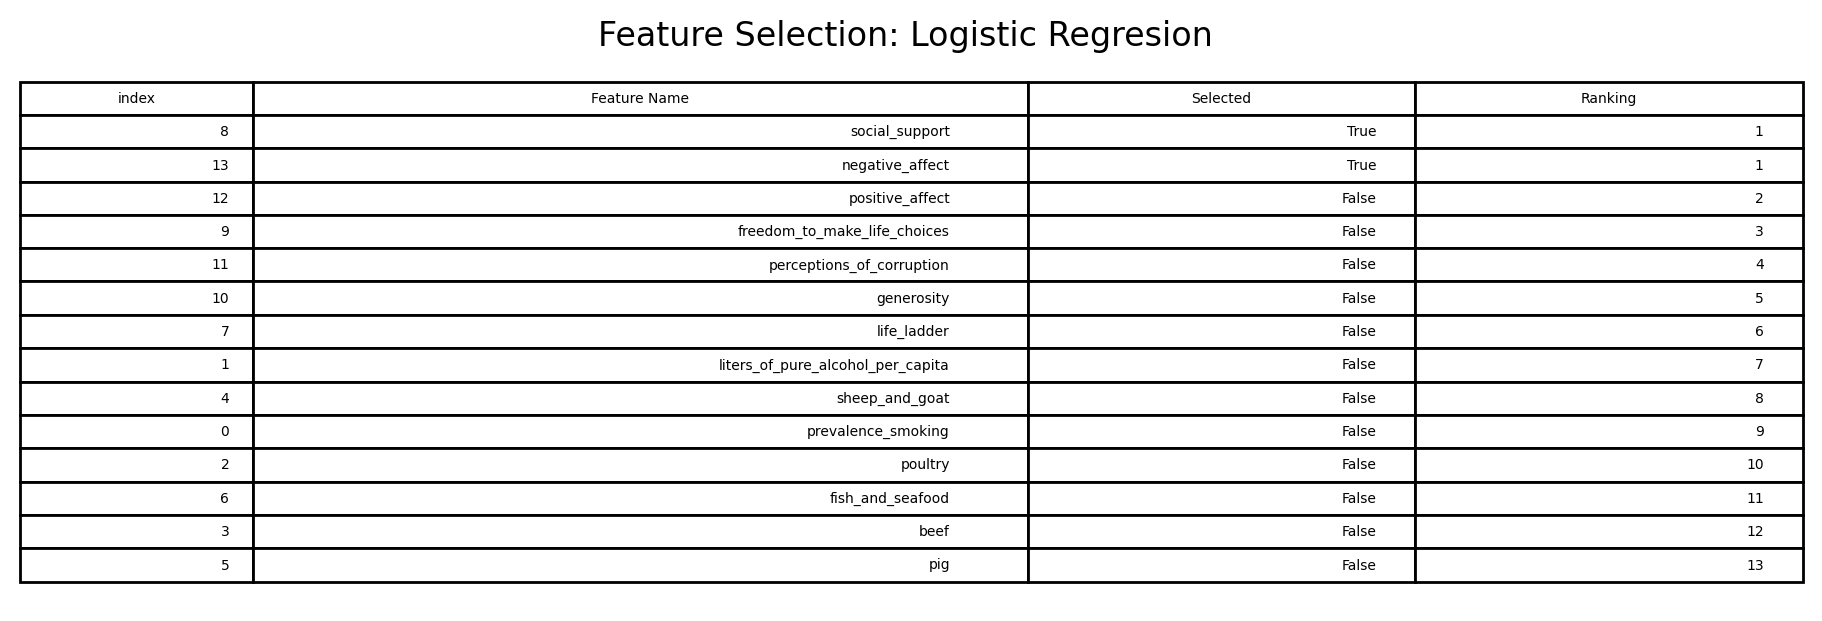
\includegraphics[scale=0.7]{images/dm_featu_sele_log_regr}
                        \caption{Feature Selection.}
                        \label{fig:dm-logistic-regression-fs-bp}
                \end{figure}


\section{Where to find this phase in the code?}

    The is a file, inside the folder python, called iteration\_three.py.
    \\
    \\
    In the line 851 there is a method that execute the whole workflow.

    \begin{verbatim}
            country_manager = ProjectManager(
                generate_images_du_02=True,
            )
            country_manager.du_02()
            country_manager.dp_03()
            country_manager.dt_04()
            country_manager.dt_07()
    \end{verbatim}

    All the images are being generate by code and referenced by using LatEx to create this document.